% vi:ft=tex
\documentclass[utf8x,10pt,aspectratio=169]{beamer}
\usepackage{hyperref}

\mode<presentation>

\usetheme[pagenum,nosectionnum,heavyfont]{tud}
\usepackage[cache=false,outputdir=.texpadtmp]{minted}
\usepackage{graphics}

%\setbeameroption{show notes}
%\setbeamertemplate{note page}[plain]

\setbeamertemplate{footnote}
{
  \tiny
  \noindent%
  \insertfootnotemark~\insertfootnotetext
}

\titlegraphic{
	
\includegraphics[width=2cm]{img/cfaed.png}\hspace*{4.75cm}~%
	
\includegraphics[width=2cm]{img/cfaed.png}
}

\title{Extending and completing Ÿauhau}
\author{Justus Adam, supervised by Sebastian Ertel and Andres Goens}
\date{\today}
\datecity{Dresden}

 \def\insertframetitle{} 
\begin{document}

\normalsize
\maketitle

\begin{frame}[fragile]{Motivation}
	
\begin{minted}{Clojure}
(defn common-friends [x y]
  (intersection (friends-of x) (friends-of y)))

(defn friends-of [x]
  (fetch (FriendsOf. x)))
\end{minted}
\pause
\begin{itemize}[<+->]
	\item Batching, Caching and Concurrency desired
	\item Retaining concise and straight forward code
\end{itemize}

\end{frame}
\addtocounter{framenumber}{-1}
\begin{frame}[fragile]
	\frametitle{Motivation}
	
\begin{minted}{Clojure}
(defalgo common-friends [x y]
  (intersection (friends-of x) (friends-of y)))

(defalgo friends-of [x]
  (fetch (mk-req (FriendsOf. x) data-source)))
\end{minted}
\begin{itemize}
	\item Batching, Caching and Concurrency desired
	\item Retaining concise and straight forward code
	\item Ÿauhau solves issue with minimal difference in code
\end{itemize}

\end{frame}

\begin{frame}{Goals}
	\pause
	\begin{block}{Current status}
		\begin{itemize}[<+->]
			\item Ÿauhau supports a base transformation on a data flow graph
			\item The structure of the graph does not reflect control flow
		\end{itemize}
	\end{block}
	\pause
	\begin{block}{Tasks}
		\begin{itemize}[<+->]
			\item Handling control flow
			\item Iteration/mapping with \texttt{smap}
			\item Conditional execution with \texttt{if}
			\item Semantics of side effects (writes), especially across algorithms
		\end{itemize}
	\end{block}
\end{frame}

\begin{frame}{Table of content}	
	\tableofcontents
\end{frame}

\section{Application}

\begin{frame}{Application}
	\begin{itemize}
		\item<2-> Large scale, distributed systems
		\item<3-> Problem first approached by Facebook for spam fighting
		\item<4-> write simple and straight forward code and still get performant results
		\item<5-> Haskell library Haxl\footnote{Simon Marlow, Louis Brandy, Jonathan Coens, and Jon Purdy. 2014. There is no fork: an abstraction for efficient, concurrent, and concise data access.}
		\item<5-> Clojure library Muse\footnote{https://goo.gl/masrsz}
		\item<5-> Scala implementation Snitch by Twitter\footnote{https://www.youtube.com/watch?v=VVpmMfT8aYw} (closed source)
	\end{itemize}
\end{frame}

\section{Ÿauhau Overview}

\begin{frame}{Ÿauhau Overview -- Ohua}
	\begin{itemize}[<+->]
		\item Ÿauhau is built on Ohua
		\item Parallelisation framework based on data flow
		\item Stateful functions and algorithms as abstraction
	\end{itemize}
\end{frame}

\begin{frame}[fragile]{Base transformation}
	
	\begin{columns}[T]
		\column{.4\textwidth}
		\begin{itemize}
			\item<2-> Rewrites high level algorithms
		\end{itemize}	
		\column{.6\textwidth}
\begin{minted}{Clojure}
(defalgo common-friends [x y]
  (intersection 
    (friends-of x) 
    (friends-of y)))

(defalgo friends-of [x]
  (fetch (mk-req (FriendsOf. x) 
                 data-source)))
\end{minted}
	\end{columns}
	
\end{frame}

\addtocounter{framenumber}{-1}

\begin{frame}[fragile]{Ÿauhau base transformation}
	
	\begin{columns}[T]
		\column{.4\textwidth}
		\begin{itemize}
			\item Rewrites high level algorithms
			\item Operates on data flow ir
		\end{itemize}	
		\column{.6\textwidth}
		\begin{minted}{Clojure}
(let [[x y] (algo-in)
      a (mk-req (FriendsOf. x) data-source)
      b (mk-req (FriendsOf. y) data-source)
      c (fetch a)
      d (fetch b)
      e (intersection a b)
  e)
		\end{minted}
	\end{columns}
	
\end{frame}

\addtocounter{framenumber}{-1}

\begin{frame}[fragile]{Ÿauhau base transformation}
	
	\begin{columns}[T]
		\column{.4\textwidth}
		\begin{itemize}
			\item Rewrites high level algorithms
			\item Operates on data flow ir
			\item Traverses data flow graph along dependencies
			\item<2-> Collect fetches, replace with accumulator
			\item<3-> Transformation is very simple and naive
		\end{itemize}	
		\column{.6\textwidth}
		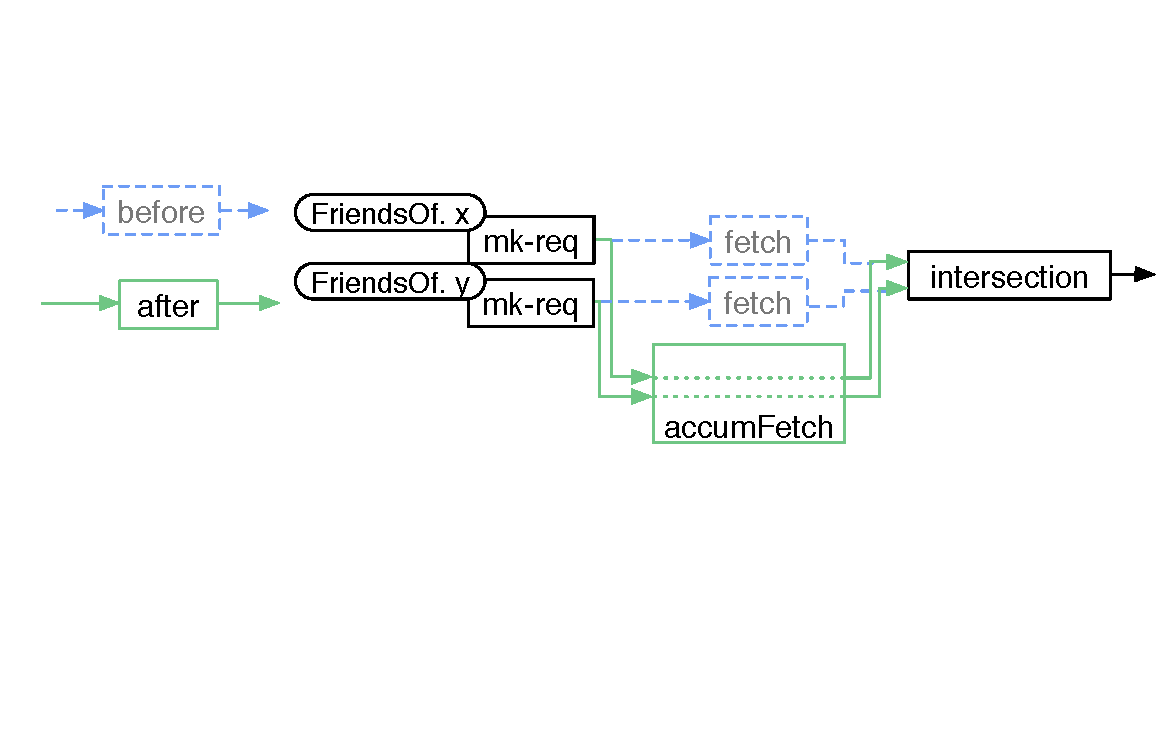
\includegraphics[width=\textwidth]{graphs/yauhau-transformation}
	\end{columns}
	
\end{frame}

\section{\texttt{smap} rewrite}
\begin{frame}{\texttt{smap} rewrite}
	\begin{columns}
		\column{0.4\textwidth}	
		\begin{itemize}
			\item<2-> Split inner graph around fetch
			\item<3-> insert \texttt{collect} and \texttt{smap} around fetch
		\end{itemize}
		\column{0.6\textwidth}
		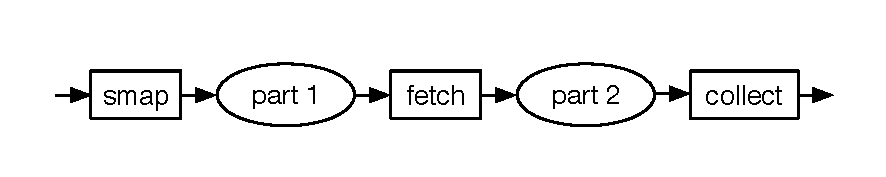
\includegraphics[width=\textwidth]{graphs/smap-rewrite-original}
	\end{columns}
		
\end{frame}

\addtocounter{framenumber}{-1}

\begin{frame}{\texttt{smap} rewrite}
	\begin{columns}
		\column{0.4\textwidth}	

		\begin{itemize}
			\item Split inner graph around fetch
			\item insert \texttt{collect} and \texttt{smap} around fetch
			\item Build tree of requests
		\end{itemize}
		\column{0.6\textwidth}
		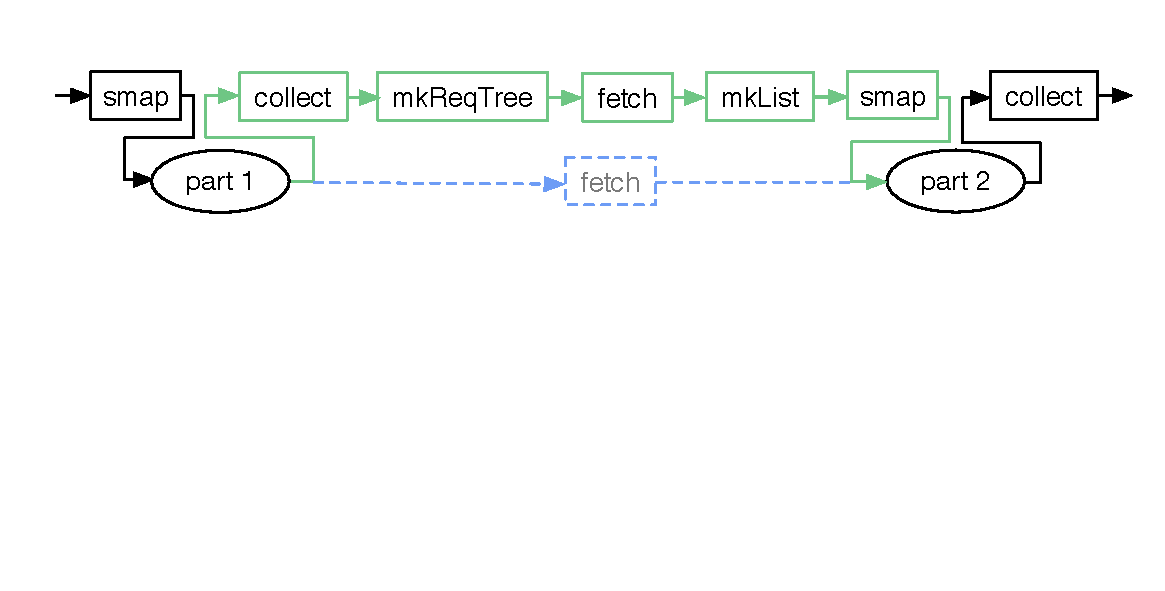
\includegraphics[width=\textwidth]{graphs/smap-rewrite}
	\end{columns}
		
\end{frame}
\section{\texttt{if} rewrite}
\begin{frame}{\texttt{if} rewrite}
	\begin{columns}
		\column{0.4\textwidth}
		\begin{itemize}[<+->]
			\item Split inner graph around fetch
			\item Replace two fetches with one being selectively given the active request
			\item Push result to the continuation of the active branch using the initial condition
			\item Inserts \texttt{identity} operators to preserve destructuring
		\end{itemize}
		\column{0.6\textwidth}
		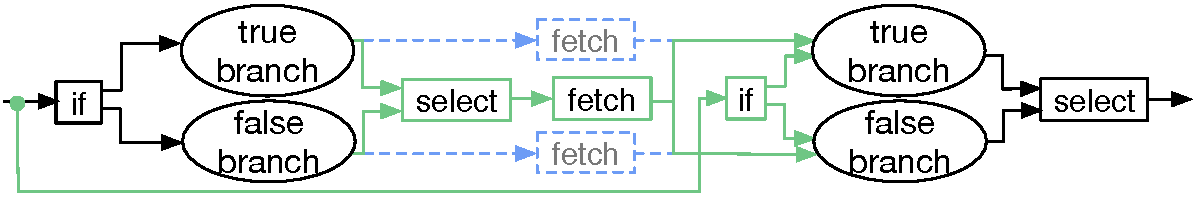
\includegraphics[width=\textwidth]{graphs/basic-if-rewrite}
	\end{columns}
\end{frame}

\addtocounter{framenumber}{-1}

\begin{frame}{\texttt{if} rewrite}
	\begin{columns}
		\column{0.4\textwidth}
		\begin{itemize}[<+->]
			\item Problem if unequal number of fetches on branches
			\item Solution: Insert extra fetches
		\end{itemize}
		\column{0.6\textwidth}
		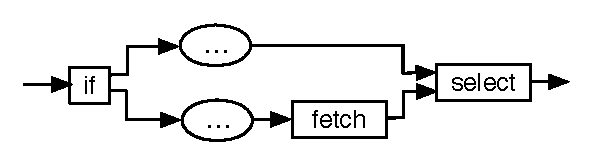
\includegraphics[width=\textwidth]{graphs/insert-empty-fetches}
	\end{columns}
\end{frame}
%
\addtocounter{framenumber}{-1}

\begin{frame}{\texttt{if} rewrite}
	\begin{columns}
		\column{0.4\textwidth}
		\begin{itemize}
			\item Problem if unequal number of fetches on branches
			\item Solution: Insert extra fetches
			\item Use NoOp (empty) requests
		\end{itemize}
		\column{0.6\textwidth}
		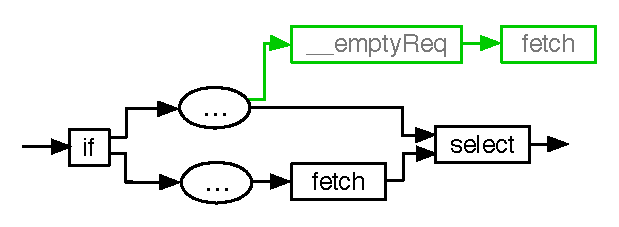
\includegraphics[width=\textwidth]{graphs/insert-empty-fetches-inserted}
	\end{columns}
\end{frame}
\section{Generalising to Context}
\begin{frame}{Generalising to Context}
	\begin{itemize}[<+->]
		\item Handle arbitrary graphs with conditionals, maps etc
		\item These structures are often interleaved
		\item Ease handling of complex nested stacks
	\end{itemize}
\end{frame}

\begin{frame}{Context}
	\begin{itemize}[<+->]
		
		\item Hidden graph structures unified into context
		\item Context is property of subgraphs emerging from node labels
		\item Inherited property
		\item Subcontexts are always fully enclosed
			
	\end{itemize}
\end{frame}

\begin{frame}{Finding context}
	
	\begin{itemize}
		\item Context recognition is done at compile time
		\item If a context opening node is found annontate subgraph
		\item Resolve full context stack by following the parent context references
		\item Hinges on the ``fully enclosing'' property
	\end{itemize}
	
\end{frame}

\begin{frame}{Handling arbitrary graphs}
	
	\begin{itemize}
		\item Calculate contexts for each fetch
		\item Contexts are unwound in order of descending nesting level
		\item Unwinding is interleaved
	\end{itemize}
\end{frame}
\section{Side Effect Semantics}
\begin{frame}[fragile]{Side Effects in Algorithms}
	\begin{columns}
		\column{0.4\textwidth}
		\begin{itemize}
			\item Execution order depends entirely on data dependencies
		\end{itemize}
		\column{0.6\textwidth}
		\begin{minted}{Clojure}
(defalgo main []
  (let [write-result 
        (write (WriteReq. "my-data") 
               data-source)
        fetch-data 
        (fetch (mk-req (Payload. "constant") 
               data-source))]
    (compute fetch-data write-result)))
		\end{minted}
		
	\end{columns}
\end{frame}

\begin{frame}{Side Effects in Algorithms}
	\begin{columns}
		\column{0.4\textwidth}
		\begin{itemize}
			\item Execution order depends entirely on data dependencies
		\end{itemize}
		\column{0.6\textwidth}
		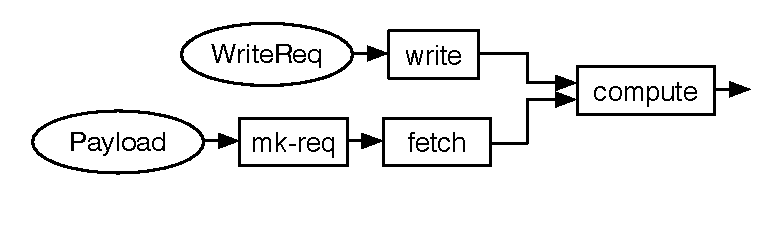
\includegraphics[width=\textwidth]{graphs/write-semantics-base}
		
	\end{columns}
\end{frame}

\begin{frame}[fragile]{Seq}
	\begin{columns}
		\column{0.4\textwidth}
		\begin{itemize}
			\item Execution order depends entirely on data dependencies
			\item Can be enforced using \texttt{seq} operator
		\end{itemize}
		\column{0.6\textwidth}
		\begin{minted}{Clojure}
(defalgo main []
  (let [write-result 
        (write (WriteReq. "my-data") 
               data-source)
        enforced 
        (seq write-result 
             (fetch (mk-req 
                      (Payload. "constant") 
                      data-source)))]
    (compute enforced write-result)))
		\end{minted}
		
	\end{columns}
\end{frame}

\begin{frame}[fragile]{Side Effects across Algorithms}
	\begin{columns}
		\column{0.4\textwidth}
		
		\begin{itemize}
			\item Execution order depends entirely on data dependencies
			\item Can be enforced using \texttt{seq} operator
			\item Not practical across algorithm boundaries
		\end{itemize}
		
		\column{0.6\textwidth}
		\begin{minted}{Clojure}
(defalgo does-read [x]
  (compute 
    (fetch (mk-req (Payload. "constant") 
                   data-source)) 
    x))
(defalgo does-write []
  (write (WriteReq. "my-data") data-source)
  ...)
(defalgo main []
  (does-read (does-write))
		\end{minted}
		
	\end{columns}
\end{frame}

\begin{frame}{Enforcing Execution Order}

	\begin{itemize}[<+->]
		\item Exploring and evaluating different approaches
		\item Combining expected semantics and efficiency
	\end{itemize}
	
	\pause
	
	\begin{block}{Current approach}
		\begin{itemize}
			\item \texttt{seq}`ing fetches to algorithm boundary
			\item for `unconnected' fetches following writes
			\item Vice versa for `unconnected' writes following reads
		\end{itemize}
	\end{block}
	\pause
	\begin{block}{Open questions}
		\begin{itemize}
			\item Always enabled?
			\item Scope?
		\end{itemize}
	\end{block}

\end{frame}

\section{Experiments and Evaluation}

\begin{frame}{Experiments and Evaluation}
	Verifying correctness (program semantics) and performance in comparison to Haxl and Muse for:
	\begin{enumerate}
		\item Modularised graphs (functions/algorithms)
		\item Graphs with map operations (\texttt{smap})
		\item Graphs with conditionals (\texttt{if})
	\end{enumerate}
	
	This requires extensions to our random code generator to allow generation of correct code with
	
	\begin{enumerate}
		\item Randomly generated functions
		\item Map operations using randomly generated functions
		\item Conditionals, with and without forcibly prefetched branches
	\end{enumerate}
	
\end{frame}

\begin{frame}
	This is the end. Thank you for listening. \\ \\
	Slides are publicly available at \href{http://static.justus.science/presentations/extending-yauhau.pdf}{http://static.justus.science/presentations/extending-yauhau.pdf}
\end{frame}

\appendix

\begin{frame}[fragile]{Haxl Implementation details}

	\begin{columns}
	
		\column{0.4\textwidth}
		\begin{itemize}
			\item Applicative functors denote independent data fetches
			\item Monad bind retrieved data
			\item Requests are GADT's encoding result type
		\end{itemize}
		\column{0.6\textwidth}
		\begin{minted}{Haskell}
commonFriends :: Id -> Id -> GenHaxl [Id]
commonFriends x y = 
    intersection <$> friendsOf x 
                 <*> friendsOf y

friendsOf :: Id -> GenHaxl [Id]
friendsOf = dataFetch . FriendsOf
		\end{minted}		
	\end{columns}
	
\end{frame}

\begin{frame}[fragile]{Muse implementation detail}
	\begin{columns}
		\column{0.4\textwidth}
		\begin{itemize}
			\item Similar syntax to Haxl
			\item fmap/\texttt{<\$>} (\texttt{<\$>} and \texttt{<*>}), flat-map (\texttt{>>=})
			\item Uses free monad to build an AST
			\item Traverses AST to find fetch rounds
		\end{itemize}
		\column{0.6\textwidth}
		\begin{minted}{Clojure}
(defn common-friends [x y]
  (<$> intersection 
    (friends-of x) 
    (friends-of y)))

(defn friends-of [x]
  (FriendsOf. x))
  
(defrecord FriendsOf [id]
  MuseAST
  (...))
		\end{minted}
	\end{columns}

\end{frame}

\end{document}

























